\documentclass{article}

\begin{document}

\setlength{\parindent}{6ex}

\begin{figure}
    \centering
    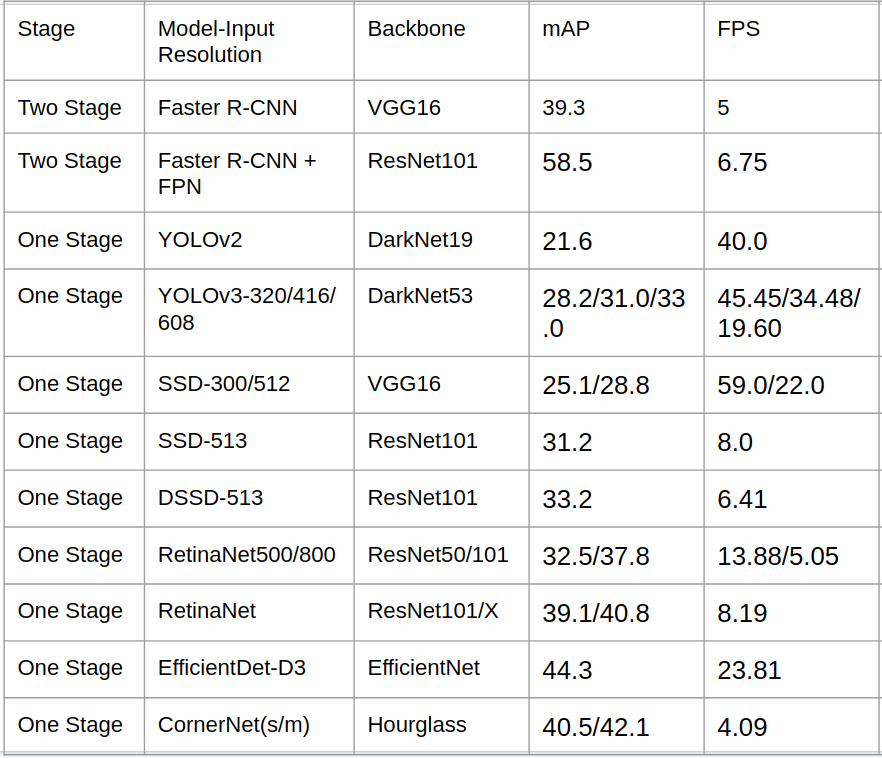
\includegraphics[width=0.8\textwidth]{performancetabledet}
    \caption{Performance table on COCO Dataset}
    \label{fig:performancetable1}
\end{figure}

\indent

Understanding the performance of detectors based on different cases and different 
features is important knowledge to decide on usage of detectors in real-life problems. 
Therefore, a table to show the performance of detectors is prepared which can be 
seen in figure \ref{fig:performancetable1}.
\end{document}